\documentclass[tikz,border=3mm,multi=tikzpicture]{standalone}
\usepackage[utf8]{inputenc}
\usepackage[T1]{fontenc}
\usepackage{helvet}
\renewcommand{\familydefault}{\sfdefault}
\usepackage{tikz}
\usetikzlibrary{angles,quotes,calc,intersections}
\begin{document}

\tikzset{every node/.append style={font=\sffamily\small}}
% TikZ 1
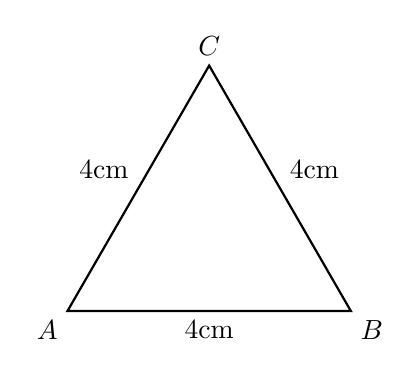
\begin{tikzpicture}[scale=1]
\coordinate (A) at (0,0); \coordinate (B) at (3.6,0); \coordinate (C) at (1.8,3.118);
\draw[thick] (A)--(B)--(C)--cycle;
\node[below left] at (A) {$A$}; \node[below right] at (B) {$B$}; \node[above] at (C) {$C$};
\node[below] at ($(A)!0.5!(B)$) {$4\mathrm{cm}$};
\node[above right] at ($(B)!0.5!(C)$) {$4\mathrm{cm}$};
\node[above left] at ($(C)!0.5!(A)$) {$4\mathrm{cm}$};
\end{tikzpicture}
% TikZ 2
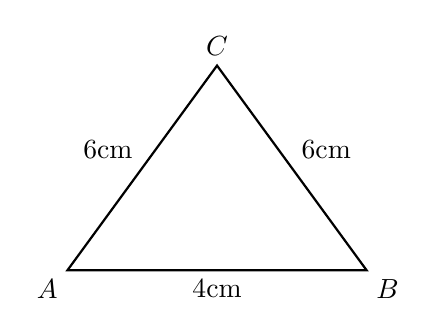
\begin{tikzpicture}[scale=1]
\coordinate (A) at (0,0); \coordinate (B) at (3.8,0); \coordinate (C) at (1.9,2.6);
\draw[thick] (A)--(B)--(C)--cycle;
\node[below left] at (A) {$A$}; \node[below right] at (B) {$B$}; \node[above] at (C) {$C$};
\node[above left] at ($(A)!0.5!(C)$) {$6\mathrm{cm}$};
\node[above right] at ($(B)!0.5!(C)$) {$6\mathrm{cm}$};
\node[below] at ($(A)!0.5!(B)$) {$4\mathrm{cm}$};
\end{tikzpicture}
% TikZ 3
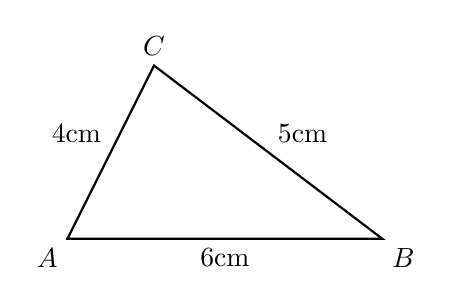
\begin{tikzpicture}[scale=1]
\coordinate (A) at (0,0); \coordinate (B) at (4,0); \coordinate (C) at (1.1,2.2);
\draw[thick] (A)--(B)--(C)--cycle;
\node[below left] at (A) {$A$}; \node[below right] at (B) {$B$}; \node[above] at (C) {$C$};
\node[below] at ($(A)!0.5!(B)$) {$6\mathrm{cm}$};
\node[above right] at ($(B)!0.5!(C)$) {$5\mathrm{cm}$};
\node[above left] at ($(C)!0.5!(A)$) {$4\mathrm{cm}$};
\end{tikzpicture}


% TikZ 4
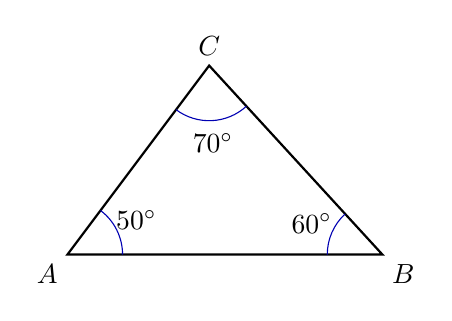
\begin{tikzpicture}[scale=1]
\coordinate (A) at (0,0); \coordinate (B) at (4,0); \coordinate (C) at (1.8,2.4);
\draw[thick] (A)--(B)--(C)--cycle;
\pic[draw=blue!70!black, "$50^{\circ}$", angle radius=7mm, angle eccentricity=1.4] {angle=B--A--C};
\pic[draw=blue!70!black, "$60^{\circ}$", angle radius=7mm, angle eccentricity=1.4] {angle=C--B--A};
\pic[draw=blue!70!black, "$70^{\circ}$", angle radius=7mm, angle eccentricity=1.4] {angle=A--C--B};
\node[below left] at (A) {$A$}; \node[below right] at (B) {$B$}; \node[above] at (C) {$C$};
\end{tikzpicture}
% TikZ 5
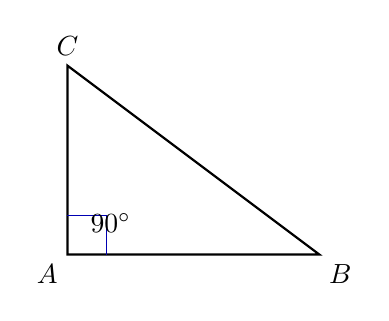
\begin{tikzpicture}[scale=1]
\coordinate (A) at (0,0); \coordinate (B) at (3.2,0); \coordinate (C) at (0,2.4);
\draw[thick] (A)--(B)--(C)--cycle;
\pic[draw=blue!70!black, angle radius=5mm] {right angle=C--A--B};
\node[below left] at (A) {$A$}; \node[below right] at (B) {$B$}; \node[above] at (C) {$C$};
\node at (0.55,0.4) {$90^{\circ}$};
\end{tikzpicture}
% TikZ 6
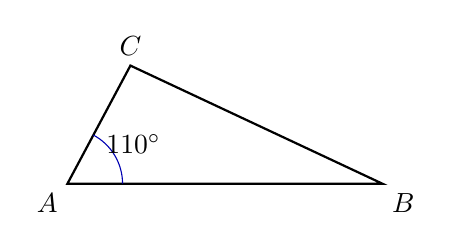
\begin{tikzpicture}[scale=1]
\coordinate (A) at (0,0); \coordinate (B) at (4,0); \coordinate (C) at (0.8,1.5);
\draw[thick] (A)--(B)--(C)--cycle;
\pic[draw=blue!70!black, "$110^{\circ}$", angle radius=7mm, angle eccentricity=1.4] {angle=B--A--C};
\node[below left] at (A) {$A$}; \node[below right] at (B) {$B$}; \node[above] at (C) {$C$};
\end{tikzpicture}
\end{document}
